\section{Spark --- Processamento Distribuído}
\label{sec:spark}

\subsection{Implementação em Java}

\subsubsection{Descrição}

Todas as versões anteriores (v2--v5) compartilham memória dentro de uma
única JVM e coordenam threads sobre um mesmo \texttt{double[][]}. A v6
substitui esse modelo por Apache Spark 4.0 em modo \texttt{local[*]}: o
dataset passa a viver como um \texttt{Dataset<Row>}/RDD particionado,
gerenciado internamente pelo Spark, e cada iteração do algoritmo é
expressa como uma transformação distribuída em vez de um laço explícito
sobre arrays. Por exigir Spark 4.0, que é testado sobre JDK 21 e não
sobre o JDK 25 usado em v1--v5, esta versão roda em um JDK diferente de
todo o restante do trabalho.

Por iteração, cada ponto é mapeado para um par
\texttt{(cluster, double[d+1])} --- onde os primeiros $d$ elementos são
as features do ponto e o último é a contagem (sempre 1,0) --- via
\texttt{mapToPair}, seguido de um \texttt{reduceByKey} que soma
localmente por partição antes de mesclar entre partições. É exatamente
o mesmo padrão de acumulação local usado por \texttt{processChunk} nas
versões v3--v5, agora expresso em operações de RDD em vez de arrays
locais explícitos. O snapshot dos centróides a cada iteração é
distribuído a todos os executores via \texttt{Broadcast<double[][]>},
ocupando o mesmo papel que o \texttt{ScopedValue}/\texttt{copy()} ocupava
nas versões anteriores.

Foram testadas duas variantes de formato de armazenamento sobre o mesmo
dataset (5,75 milhões de pontos, 38 features): uma lendo o CSV original
e outra lendo uma conversão Parquet do mesmo conteúdo. As tags
correspondentes são \texttt{v6-csv} e \texttt{v6-parquet}.

\begin{table}[H]
\centering
\begin{tabular}{lp{11cm}}
\hline
\textbf{Componente} & \textbf{Alteração} \\
\hline
\texttt{pom.xml}     & \texttt{maven.compiler.release} alterado de 25 para 21;
                       dependências de JMH, JCStress e JMeter removidas;
                       adicionados \texttt{spark-core\_2.13} e \texttt{spark-sql\_2.13} 4.0.0 \\
\texttt{KMeans.java} & reescrita completa: \texttt{SparkSession local[*]}, carga do
                       dataset via \texttt{DataFrame}, \texttt{mapToPair} + \texttt{reduceByKey}
                       por iteração, \texttt{Broadcast} do snapshot de centróides \\
\texttt{Main.java}   & remove o uso de \texttt{CsvDataset}; cronometragem por
                       \texttt{System.nanoTime()} em torno da execução completa \\
\hline
\end{tabular}
\caption{Alterações da v6 em relação à v5.}
\label{tab:v6-changes}
\end{table}

A Figura~\ref{fig:snippet-spark-iteration} mostra o laço de iteração completo:
o broadcast do snapshot de centróides seguido do par
\texttt{mapToPair}+\texttt{reduceByKey} que acumula somas e contagens por
cluster, o mesmo padrão de acumulação local das versões anteriores expresso
em operações de RDD.

\begin{figure}[H]
  \centering
  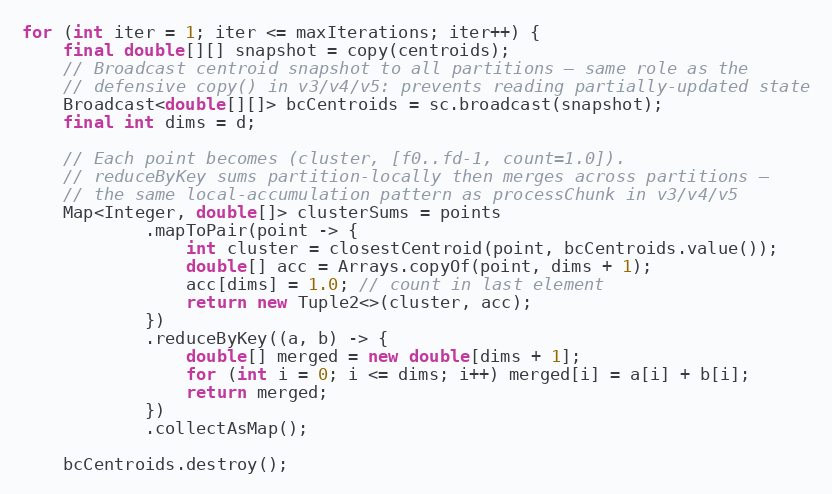
\includegraphics[width=0.85\textwidth]{img/8-spark/snippet-1}
  \caption{Broadcast do snapshot de centróides e acumulação por
           \texttt{mapToPair}+\texttt{reduceByKey} a cada iteração
           (\texttt{KMeans.cluster}, tag \texttt{v6-csv}).}
  \label{fig:snippet-spark-iteration}
\end{figure}

A Figura~\ref{fig:snippet-spark-format} mostra a única diferença de código
entre as duas variantes testadas: o formato de leitura do \texttt{DataFrame}.
Todo o restante do arquivo --- broadcast, \texttt{mapToPair}, \texttt{reduceByKey},
avaliação final --- é idêntico entre \texttt{v6-csv} e \texttt{v6-parquet}.

\begin{figure}[H]
  \centering
  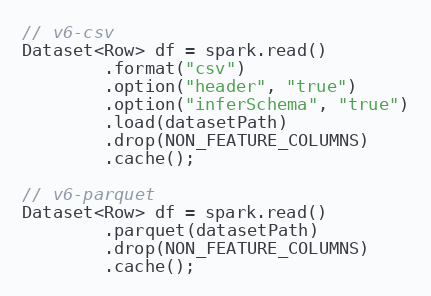
\includegraphics[width=0.7\textwidth]{img/8-spark/snippet-2}
  \caption{Única diferença de código entre \texttt{v6-csv} e
           \texttt{v6-parquet}: o formato de leitura do \texttt{DataFrame}
           (\texttt{KMeans.cluster}).}
  \label{fig:snippet-spark-format}
\end{figure}

O diagrama de classes da Figura~\ref{fig:class-diagram-spark} mostra a
estrutura da v6, bem mais simples que a das versões anteriores:
\texttt{Main} chama \texttt{KMeans.cluster}, que devolve um
\texttt{KMeansResult} (o mesmo \textit{record} usado desde a v1) e depende
diretamente de três tipos da API do Spark --- \texttt{SparkSession},
\texttt{Dataset<Row>} e \texttt{Broadcast<double[][]>}. O
\texttt{CsvDataset} das versões anteriores desaparece do grafo de
dependências: o arquivo ainda existe fisicamente no repositório da tag
\texttt{v6-csv}, mas não é mais referenciado em nenhum ponto do código.

\begin{figure}[H]
  \centering
  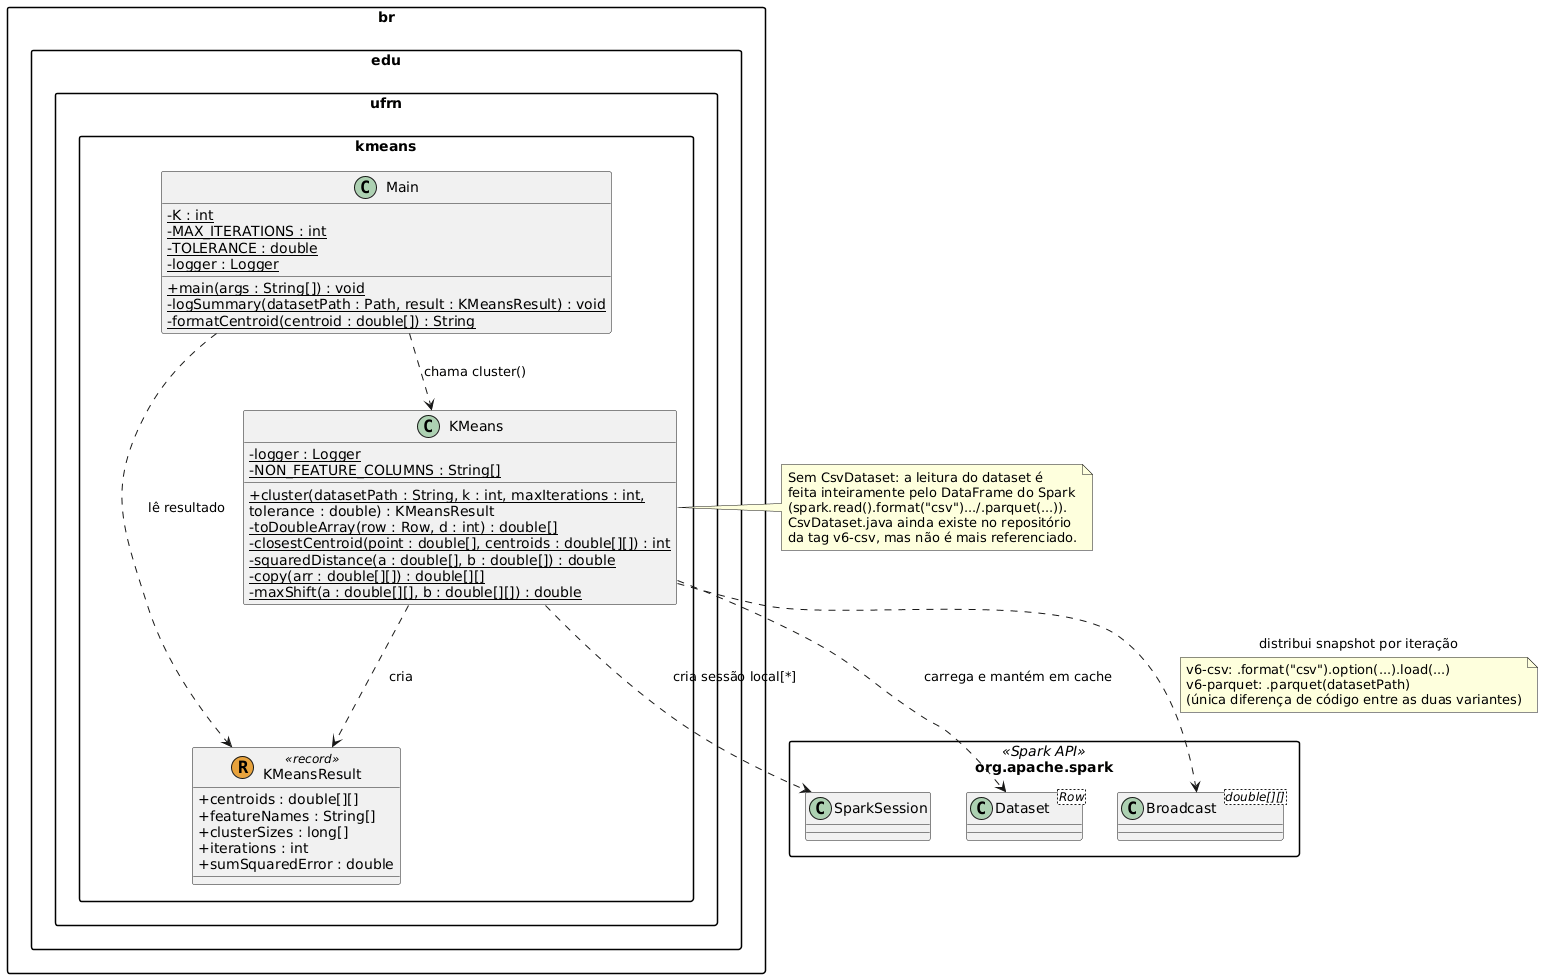
\includegraphics[width=0.95\textwidth]{img/8-spark/class-diagram}
  \caption{Diagrama de classes da v6 (Spark). \texttt{Main} e \texttt{KMeans}
           seguem estáticas como nas versões anteriores; \texttt{KMeansResult}
           é reaproveitado sem alterações. A única diferença de código entre
           \texttt{v6-csv} e \texttt{v6-parquet} está no carregamento do
           \texttt{Dataset<Row>} (ver Figura~\ref{fig:snippet-spark-format}).}
  \label{fig:class-diagram-spark}
\end{figure}

\subsubsection{Resultados}

\paragraph{Aplicabilidade das Ferramentas de Benchmark}

Nenhuma das ferramentas usadas em v1--v5 se aplica diretamente à v6.
JMH não é viável porque a inicialização de uma \texttt{SparkSession} é
pesada demais para caber no modelo de fork/iterações curtas do JMH.
JMeter não se aplica porque o Spark não foi projetado para atender
chamadas concorrentes de alta frequência --- rodar JMeter contra uma
única sessão Spark compartilhada testaria o escalonador do Spark, não o
algoritmo. JCStress não se aplica porque o modelo de execução do Spark
não tem estado mutável compartilhado entre tarefas por construção --- não
há região crítica para testar. As métricas usadas nesta versão são
\textbf{tempo de parede} (\texttt{System.nanoTime()} em torno da
execução completa) e \textbf{profile JFR}, complementado pela Spark UI
(\texttt{http://localhost:4040}) para inspeção do DAG de jobs e stages.

\paragraph{Avaliação de Tempo de Parede}

Ambas as variantes foram executadas com $k=10$ e \texttt{maxIter}=10
(sem convergência dentro desse limite), sobre o mesmo dataset de 5,75
milhões de pontos e 38 features.

\begin{table}[H]
\centering
\begin{tabular}{lrr}
\hline
\textbf{Variante} & \textbf{Tempo total (ms)} & \textbf{Tempo/iter.\textsuperscript{*} (s)} \\
\hline
v6-csv     & 34.624 & 3{,}46 \\
v6-parquet & 44.264 & 4{,}43 \\
\hline
\end{tabular}
\caption{Tempo de parede --- v6-csv vs.\ v6-parquet ($k=10$, \texttt{maxIter}=10,
mesmo dataset de 5,75 milhões de pontos; SSE final praticamente idêntico
entre as duas variantes, ver texto).
\textsuperscript{*}Estimado como tempo total $\div$ 10 iterações; não é uma
medição isolada como o B2 do JMH nas versões anteriores, apenas uma
referência aproximada de ordem de grandeza.}
\label{tab:wallclock-v6}
\end{table}

O SSE final é praticamente idêntico entre as duas variantes ---
confirmando que ambas processam o mesmo dataset e chegam ao mesmo
resultado, como esperado, já que a única diferença de código entre elas
é o formato de leitura do \texttt{DataFrame}. Contra a expectativa comum
de que um formato colunar e comprimido como o Parquet seria mais rápido
de ler que texto puro, o \textbf{Parquet ficou \textasciitilde28\% mais
lento que o CSV} nesta carga (44.264 ms contra 34.624 ms). A seção de
profile a seguir explica a causa.

\paragraph{Avaliação de Profile}

\textbf{v6-csv.} A gravação JFR totalizou 11.263 amostras de execução.

\begin{table}[H]
\centering
\small
\begin{tabular}{p{7.4cm}rrp{3cm}}
\hline
\textbf{Método} & \textbf{Amostras} & \textbf{CPU (\%)} & \textbf{Categoria} \\
\hline
\texttt{KMeans.squaredDistance}       & 1475 & 13{,}1 & Algoritmo \\
\texttt{CharInputReader.getString}    & 1179 & 10{,}5 & Parsing CSV (univocity) \\
\texttt{CompressibleColumnBuilder}    &  621 &  5{,}5 & Cache colunar (Spark) \\
\texttt{HashMap.put0}                 &  413 &  3{,}7 & Overhead Scala/Spark \\
\texttt{KMeans.closestCentroid}       &  352 &  3{,}1 & Algoritmo \\
\texttt{LineReader.readDefaultLine}   &  330 &  2{,}9 & Parsing CSV (Hadoop) \\
\hline
\end{tabular}
\caption{Hot methods na v6-csv (JFR, 11.263 amostras).}
\label{tab:jfr-hot-v6-csv}
\end{table}

Diferente da v3 --- onde nenhum evento de leitura de dataset aparece
depois da carga inicial ---, os frames de \textit{parsing} de CSV
(\texttt{AbstractCharInputReader}, \texttt{LineReader}) seguem entre os
mais amostrados mesmo depois da carga inicial. O motivo aparece na saída
de execução: o Spark registra repetidos avisos
\texttt{MemoryStore - Not enough space to cache rdd\_X in memory!} ---
sob os 4 GB de memória do driver, nem todas as partições do dataset
cabem no cache, e as partições que não couberam são \textbf{relidas e
reparseadas do CSV a cada iteração} em vez de servidas da memória. Isso
é uma diferença estrutural importante frente à v3: lá, o dataset ou cabe
inteiro no heap ou a JVM falha; aqui, o cache do Spark degrada
silenciosamente para recomputação sob pressão de memória, sem erro
explícito.

\textbf{v6-parquet.} A gravação JFR totalizou 11.016 amostras de execução.

\begin{table}[H]
\centering
\small
\begin{tabular}{p{7.4cm}rrp{3cm}}
\hline
\textbf{Método} & \textbf{Amostras} & \textbf{CPU (\%)} & \textbf{Categoria} \\
\hline
\texttt{KMeans.squaredDistance}       & 2152 & 19{,}5 & Algoritmo \\
\texttt{ParquetDictionary.decodeToLong} & 912 &  8{,}3 & Decodificação Parquet \\
\texttt{CodegenIterator.processNext}  &  813 &  7{,}4 & Codegen (Spark) \\
\texttt{CompressibleColumnBuilder}    &  757 &  6{,}9 & Cache colunar (Spark) \\
\texttt{HashMap.findNode}             &  659 &  6{,}0 & Overhead Scala/Spark \\
\texttt{KMeans.closestCentroid}       &  603 &  5{,}5 & Algoritmo \\
\texttt{ParquetDictionary.decodeToDouble} & 442 & 4{,}0 & Decodificação Parquet \\
\hline
\end{tabular}
\caption{Hot methods na v6-parquet (JFR, 11.016 amostras).}
\label{tab:jfr-hot-v6-parquet}
\end{table}

Os mesmos avisos de pressão de memória aparecem no log do v6-parquet,
mas com um comportamento diferente: em vez de descartar o bloco que não
coube, o \texttt{BlockManager} registra \texttt{"Persisting block to
disk instead"} --- o formato colunar e comprimido do Parquet muda a
forma como o Spark decide lidar com a falta de espaço no cache. Ainda
assim, o tempo total foi maior: a decodificação de dicionário/delta do
Parquet (\texttt{ParquetDictionary.decodeToLong}/\texttt{decodeToDouble})
soma uma fração relevante das amostras, um custo de CPU real que o CSV
--- apesar de mais lento para ler bruto --- não paga da mesma forma
depois que uma partição está em cache.

\textbf{Heap e GC.} O pico de heap foi de 3.891,2 MB
(\textasciitilde3,89 GB) na v6-csv e 3.993,6 MB (\textasciitilde3,99 GB)
na v6-parquet --- ambos notavelmente acima dos \textasciitilde2,6--2,76
GB de v3/v4/v5, apesar de operarem sobre o mesmo dataset bruto: as
estruturas internas do Spark (representação colunar em cache, overhead
de execução distribuída no driver e nos executores locais) somam
memória real acima dos dados em si, e ambas as variantes ficam próximas
do teto configurado de 4 GB (\texttt{-Xmx4g}) --- consistente com os
avisos de pressão de cache já discutidos. A v6-csv registrou 243
coletas de GC e a v6-parquet 124; esses números não são diretamente
comparáveis aos das versões anteriores, pois incluem sobrecarga do
próprio Spark/JVM além do algoritmo.

\subsection{Discussão}

O Spark é, neste dataset e nesta escala, \textbf{mais lento que
v3/v4/v5}: o tempo por iteração aproximado (3,46 s na v6-csv, 4,43 s na
v6-parquet) fica bem acima do B2 de v3/v4/v5 (1,60--1,98 s). O dataset
inteiro cabe confortavelmente em memória numa única máquina, e o custo
de serialização, broadcast e gerenciamento de partições distribuídas do
Spark supera qualquer benefício que o processamento distribuído
ofereceria numa escala maior. O valor pedagógico desta versão está na
mudança radical de modelo de programação --- de threads coordenadas
sobre memória compartilhada para transformações distribuídas sobre um
\texttt{Dataset} particionado --- não em um ganho de desempenho.

A comparação entre CSV e Parquet dentro da própria v6 é o achado mais
interessante desta seção: contra a intuição comum de que um formato
colunar e comprimido seria mais rápido, o \textbf{Parquet foi
\textasciitilde28\% mais lento} nesta carga, porque o custo de
decodificação de dicionário/delta por linha supera a economia de
I/O bruto. É o mesmo tipo de lição que o profile da versão serial já
havia ensinado --- \textbf{medir antes de assumir} --- agora aplicada à
escolha de formato de armazenamento em vez de à escolha de estratégia de
concorrência.

Por fim, a v6 expõe um modo de falha que nenhuma versão single-JVM tem:
sob pressão de memória, o cache do Spark degrada silenciosamente para
recomputação (relendo/reparseando partições, como visto na v6-csv) em
vez de falhar de forma explícita. Na v3, o dataset ou cabe inteiro no
heap ou a JVM lança \texttt{OutOfMemoryError} --- uma falha visível e
imediata. No Spark, a mesma restrição de memória se manifesta como uma
degradação de desempenho silenciosa, que só fica evidente ao inspecionar
o profile ou os logs de aviso do \texttt{MemoryStore}.
